%%% Для сборки выполнить 2 раза команду: pdflatex <имя файла>

\documentclass[a4paper,12pt]{article}

\usepackage{ucs}
\usepackage[utf8x]{inputenc}
\usepackage[russian]{babel}
%\usepackage{cmlgc}
\usepackage{graphicx}
\usepackage{hyperref}
\usepackage{listings}
\usepackage{xcolor}
%\usepackage{courier}

\makeatletter
\renewcommand\@biblabel[1]{#1.}
\makeatother

\newcommand{\myrule}[1]{\rule{#1}{0.4pt}}
\newcommand{\sign}[2][~]{{\small\myrule{#2}\\[-0.7em]\makebox[#2]{\it #1}}}

% Поля
\usepackage[top=20mm, left=30mm, right=10mm, bottom=20mm, nohead]{geometry}
\usepackage{indentfirst}

% Межстрочный интервал
\renewcommand{\baselinestretch}{1.50}


\begin{document}

%%%%%%%%%%%%%%%%%%%%%%%%%%%%%%%
%%%                         %%%
%%% Начало титульного листа %%%

\thispagestyle{empty}
\begin{center}


\renewcommand{\baselinestretch}{1}
{\large
{\sc Петрозаводский государственный университет\\
Институт математики и информационных технологий\\
	Кафедра Информатики и Математического Обеспечения
}
}

\end{center}


\begin{center}
%%%%%%%%%%%%%%%%%%%%%%%%%
%
% Раскомментируйте (уберите знак процента в начале строки)
% для одной из строк типа направления  - бакалавриат/
% магистратура и для одной из
% строк Вашего направление подготовки
%
% Направление подготовки бакалавриата \\
% 01.03.02 Прикладная математика и информатика \\
% 09.03.02 - Информационные системы и технологии \\
09.03.04 - Программная инженерия \\
% Направление подготовки магистратуры \\
% 01.04.02 - Прикладная математика и информатика \\
% 09.04.02 - Информационные системы и  технологии \\
%
% 
%%%%%%%%%%%%%%%%%%%%%%%%%
	% \textcolor{red}{<Ваши тип и направление подготовки>} 
\end{center}

\vfill

\begin{center}
{\normalsize Отчет о проектной работе по курсу <<Разработка приложений для мобильных ОС>>} \\

\medskip

%%% Название работы %%%
	{\Large \sc Приложение <<Remote Control>>} \\
	% (промежуточный)
\end{center}

\medskip

\begin{flushright}
\parbox{11cm}{%
\renewcommand{\baselinestretch}{1.2}
\normalsize
	Выполнила:\\
Квист Татьяна Денисовна\\
студентка 2 курса группы 22207
\begin{flushright}
	Т. Д. Квист \sign[подпись]{4cm}
\end{flushright}

Руководитель:\\
А. В. Бородин, старший преподаватель \\
% \begin{flushright}
% \sign[подпись]{4cm}
% \end{flushright}

}
\end{flushright}

\vfill

\begin{center}
\large
    Петрозаводск --- 2021-2022
\end{center}

%%% Конец титульного листа  %%%
%%%                         %%%
%%%%%%%%%%%%%%%%%%%%%%%%%%%%%%%

%%%%%%%%%%%%%%%%%%%%%%%%%%%%%%%%
%%%                          %%%
%%% Содержание               %%%

\newpage

\hypersetup{hidelinks}
\tableofcontents

\newpage
\section*{Введение}
\addcontentsline{toc}{section}{Введение}


Цель проекта: разработать мобильное приложение для дистанционного управления светодиодной лентой. \\

Задачи проекта: 
\begin{enumerate}
    \item Разработать модуль главной страницы;
    \item Разработать модуль для выбора монотонной подсветки;
    \item Разработать модуль для создания цветовой последовательности;
    \item Разработать модуль для выбора режима;
    \item Разработать модуль для создания градиента;
    \item Реализовать мобильное приложение с использованием разработанных модулей с использованием React Native и Expo.
\end{enumerate}

Всё больше и больше компаний создают предметы для умного дома. С помощью телефона можно настроить холоднильник, чайник и кофемашину. Но не стоит забывать и про интерьер, ведь от него многое зависит: как ваши гости оценят обстановку, праздничное настроение, да и настроение в целом. Поэтому предлагается создать пульт дистанционного управления для светодиодной ленты.    

%%%                          %%%
%%%%%%%%%%%%%%%%%%%%%%%%%%%%%%%%

%%%%%%%%%%%%%%%%%%%%%%%%%%%%%%%%
%%%                          %%%
%%% Требования к приложению  %%%

\section{Требования к приложению}
\begin{itemize}
    \item Корректное отображение всех элементов;
    \item Отображение выбора пользователя;
    \item Отправка данных на сервер. 
\end{itemize}

%%%                          %%%
%%%%%%%%%%%%%%%%%%%%%%%%%%%%%%%%

%%%%%%%%%%%%%%%%%%%%%%%%%%%%%%%%%
%%%                           %%%
%%% Проектирование приложения %%%
\section{Проектирование приложения}
Модули приложения:
\begin{enumerate}
    \item App.js --- основной модуль, содержащий в себе остальные модули интерфейса.
    \item Footer.js --- модуль с разделом навигации и названием приложения.
    \item Header.js --- модуль с заголовком раздела. 
    \item MonoColor.js --- модуль с выбором цвета монотонной подсветки. Состоит из нескольких других модулей:
    \begin{itemize}
        \item ColorPalette.js --- модуль для отображения группы цветов.
        \item Color.js --- модуль для отображения цвета. Круг с диаметром в 25 пикселей. В качестве аргумента получает строку с цветом (hex, rgb или название). 
    \end{itemize}
    \item Sequence.js --- модуль с выбором цветовой последовательности. Используются элементы, которые отвечают за выбор пользователя (три круга), которые меняются в зависимости от выбора. Состоит из нескольких других модулей:
    \begin{itemize}
        \item ColorPaletteSmallSeq.js --- модуль для отображения группы цветов.
        \item ColorSmall.js --- модуль для отображения цвета. Круг с диаметром в 20 пикселей. В качестве аргумента получает строку с цветом (hex, rgb или название). 
    \end{itemize}
    \item Modes.js --- модуль с выбором режима подсветки. Всего есть два режима: радуга (на каждом светодиоде одинаковый цвет в один момент времени) и горизонтальная радуга (на каждом светодиоде разный цвет в один момент времени).
    \item Gradient.js --- модуль с выбором градиента. Пользователь выбирает два цвета, из которых создаётся линейный градиент. Состоит из нескольких других модулей:
    \begin{itemize}
        \item ColorPaletteSmallGrad.js --- модуль для отображения группы цветов.
        \item ColorSmall.js 
    \end{itemize}
\end{enumerate}

%%%                          %%%
%%%%%%%%%%%%%%%%%%%%%%%%%%%%%%%%

%%%%%%%%%%%%%%%%%%%%%%%%%%%%%%%%%
%%%                           %%%
%%% Реализация приложения     %%%
\section{Релизация приложения}
Для реализации приложения был использован язык <<JavaScript>> и фреймворк <<React Native>> --- кроссплатформенный фреймворк с открытым исходным кодом для разработки нативных мобильных и настольных приложений на JavaScript и TypeScript, созданный Facebook, Inc. На его основе было разработано 12 модулей (компонентов). 

Важным моментом является адаптация под мобильные устройства, а в частности, корректное отображение для разных разрешений устройств. Для этого использовались гибкие стили (flex, wrap).    
\begin{itemize}
    \item Количество модулей: 12.
    \item Количество классов: 7.
    \item Количество <<JavaScript>> функций: 7.
    \item Количество строк <<JavaScript>> кода: 979.
\end{itemize}

%%%                          %%%
%%%%%%%%%%%%%%%%%%%%%%%%%%%%%%%%

%%%%%%%%%%%%%%%%%%%%%%%%%%%%%%%%%
%%%                           %%%
%%% Заключение                %%%

\section*{Заключение}
\addcontentsline{toc}{section}{Заключение}

В результате проекта было разработано мобильное приложение для дистанционного управления светодиодной лентой. Пользователь может выбрать монотонное освещение, последовательность цветов, уже запрограммированный режим или выбрать два цвета для линейного градиента.

Получен опыт работы с <<React Native>> и <<Expo>>.

\begin{center}
    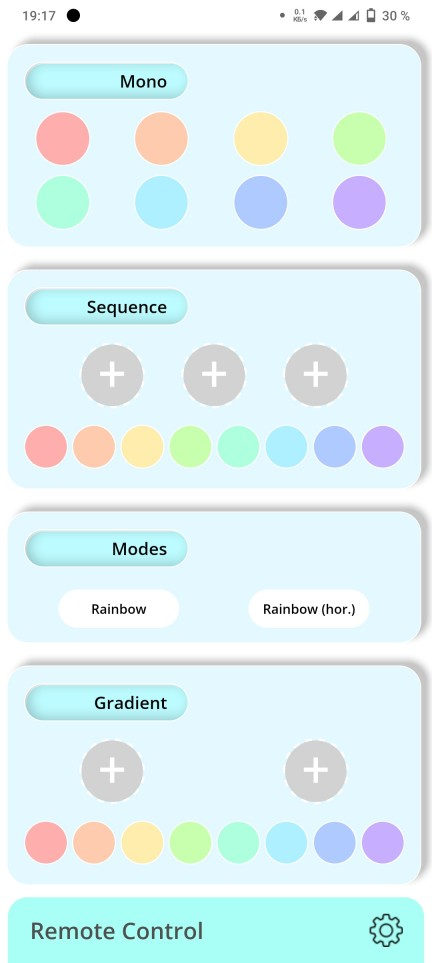
\includegraphics[width = .43\textwidth]{app.jpg}    
\end{center}

\end{document}
